\documentclass[../../main.tex]{subfiles}
\graphicspath{{\subfix{../../image/}}} % 指定图片目录,后续可以直接使用图片文件名。

% 例如:
% \begin{figure}[H]
% \centering
% \includegraphics[scale=0.4]{图.png}
% \caption{}
% \label{figure:图}
% \end{figure}
% 注意:上述\label{}一定要放在\caption{}之后,否则引用图片序号会只会显示??.

\begin{document}

\section{Lagrange插值定理}

\begin{definition}[插值基函数]
若 $n$ 次多项式 $l_j(x) (j = 0, 1, \cdots, n)$ 在 $n + 1$ 个节点 $x_0 < x_1 < \cdots < x_n$ 上满足条件 
\begin{align*}
l_j(x_k) = \begin{cases} 
1, & k = j, \\ 
0, & k \neq j 
\end{cases} \quad j, k = 0, 1, \cdots, n.
\end{align*}
就称这 $n + 1$ 个 $n$ 次多项式 $l_0(x), l_1(x), \cdots, l_n(x)$ 为节点 $x_0, x_1, \cdots, x_n$ 上的 $\boldsymbol{n}$ 次\textbf{插值基函数}。
\end{definition}

\begin{theorem}\label{theorem:插值基函数的求法}
证明:节点 $x_0, x_1, \cdots, x_n$ 上的$n$ 次插值基函数为 
\begin{align}
l_k(x) = \frac{(x - x_0) \cdots (x - x_{k - 1})(x - x_{k + 1}) \cdots (x - x_n)}{(x_k - x_0) \cdots (x_k - x_{k - 1})(x_k - x_{k + 1}) \cdots (x_k - x_n)}, \quad k = 0, 1, \cdots, n .\label{eq:::::-----------48--2.8}
\end{align}
\end{theorem}
\begin{proof}
下面先讨论$n = 1$ 的简单情形,此时假定给定区间 $[x_k, x_{k + 1}]$ 及端点函数值 $y_k = f(x_k)$,$y_{k + 1} = f(x_{k + 1})$,要求线性插值多项式 $L_1(x)$,使它满足 
\[
L_1(x_k) = y_k, \quad L_1(x_{k + 1}) = y_{k + 1}
\]
$y = L_1(x)$ 的几何意义就是通过两点 $(x_k, y_k)$ 与 $(x_{k + 1}, y_{k + 1})$ 的直线,如\reffig{figure:线性插值基函数示例图}所示,$L_1(x)$ 的表达式可由几何意义直接给出 
\begin{align*}
\begin{cases} 
L_1(x) = y_k + \frac{y_{k + 1} - y_k}{x_{k + 1} - x_k}(x - x_k) \quad \text{(点斜式)}, \\ 
L_1(x) = \frac{x_{k + 1} - x}{x_{k + 1} - x_k} y_k + \frac{x - x_k}{x_{k + 1} - x_k} y_{k + 1} \quad \text{(两点式)} 
\end{cases}
\end{align*}
由两点式看出,$L_1(x)$ 是由两个线性函数 
\[
l_k(x) = \frac{x - x_{k + 1}}{x_k - x_{k + 1}}, \quad l_{k + 1}(x) = \frac{x - x_k}{x_{k + 1} - x_k} .
\]
线性组合得到的,其系数分别为 $y_k$ 及 $y_{k + 1}$,即 
\[
L_1(x) = y_k l_k(x) + y_{k + 1} l_{k + 1}(x).
\]
显然,$l_k(x)$ 及 $l_{k + 1}(x)$ 也是线性插值多项式,在节点 $x_k$ 及 $x_{k + 1}$ 上分别满足条件 
\[
l_k(x_k) = 1, \quad l_k(x_{k + 1}) = 0;
\]
\[
l_{k + 1}(x_k) = 0, \quad l_{k + 1}(x_{k + 1}) = 1
\]
我们称函数 $l_k(x)$ 及 $l_{k + 1}(x)$ 为{\heiti 线性插值基函数},它们的图形见\reffig{figure:线性插值基函数示例图}。
\begin{figure}[H]
\centering
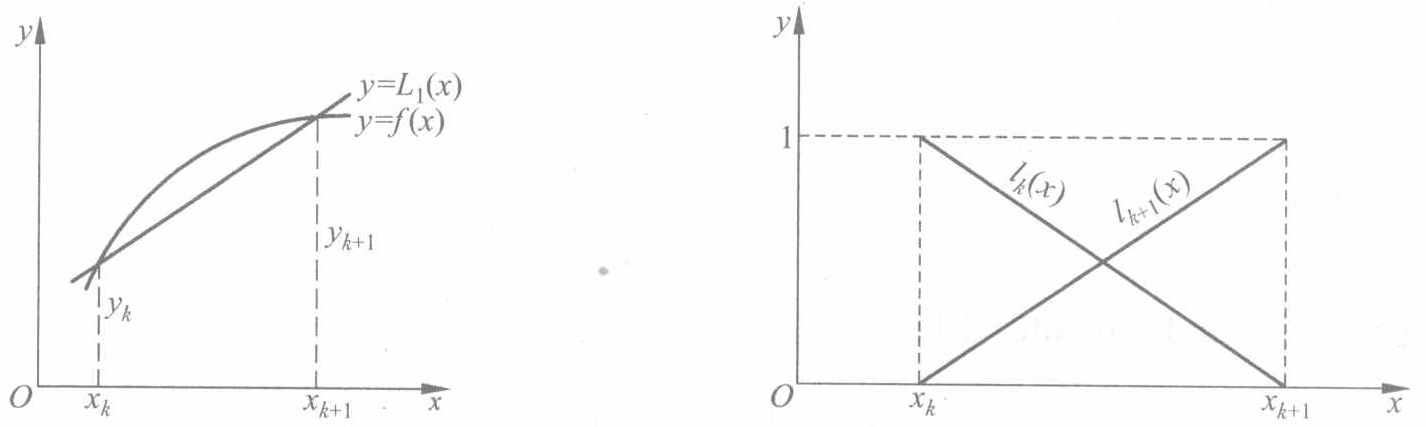
\includegraphics[scale=0.4]{线性插值基函数示例图.png}
\caption{}
\label{figure:线性插值基函数示例图}
\end{figure}
下面讨论 $n = 2$ 的情况。此时假定插值节点为 $x_{k - 1}, x_k, x_{k + 1}$,要求二次插值多项式 $L_2(x)$,使它满足 
\[
L_2(x_j) = y_j, \quad j = k - 1, k, k + 1
\]
我们知道 $y = L_2(x)$ 在几何上就是通过三点 $(x_{k - 1}, y_{k - 1})$,$(x_k, y_k)$,$(x_{k + 1}, y_{k + 1})$ 的抛物线。为了求出 $L_2(x)$ 的表达式,可采用基函数方法,此时基函数 $l_{k - 1}(x), l_k(x)$ 及 $l_{k + 1}(x)$ 是二次函数,且在节点上分别满足条件
\begin{align*}
\begin{cases}
l_{k-1}(x_{k-1})=1,		l_{k-1}(x_j)=0,		&j=k,k+1;\\
l_k(x_k)=1,		l_k(x_j)=0,		&j=k-1,k+1;\\
l_{k+1}(x_{k+1})=1,		l_{k+1}(x_j)=0,		&j=k-1,k\\
\end{cases}
\end{align*}
满足上述条件的插值基函数是很容易求出的,例如求 $l_{k - 1}(x)$,因它有两个零点 $x_k$ 及 $x_{k + 1}$,故可表示为
\[
l_{k - 1}(x) = A(x - x_k)(x - x_{k + 1})
\]
其中 $A$ 为待定系数,可由条件 $l_{k - 1}(x_{k - 1}) = 1$ 定出 
\[
A = \frac{1}{(x_{k - 1} - x_k)(x_{k - 1} - x_{k + 1})}.
\]
于是
\[
l_{k - 1}(x) = \frac{(x - x_k)(x - x_{k + 1})}{(x_{k - 1} - x_k)(x_{k - 1} - x_{k + 1})}.
\]
同理可得 
\[
l_k(x) = \frac{(x - x_{k - 1})(x - x_{k + 1})}{(x_k - x_{k - 1})(x_k - x_{k + 1})},
\]
\[
l_{k + 1}(x) = \frac{(x - x_{k - 1})(x - x_k)}{(x_{k + 1} - x_{k - 1})(x_{k + 1} - x_k)}.
\]
二次插值基函数 $l_{k - 1}(x), l_k(x), l_{k + 1}(x)$ 在区间 $[x_{k - 1}, x_{k + 1}]$ 上的图形见\reffig{figure:二次插值基函数示例图}。
\begin{figure}[H]
\centering
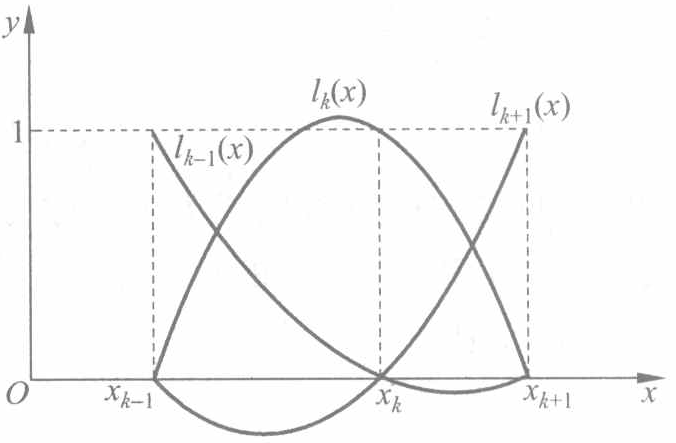
\includegraphics[scale=0.4]{二次插值基函数示例图.png}
\caption{}
\label{figure:二次插值基函数示例图}
\end{figure}
对 $n = 1$ 及 $n = 2$ 时的情况上述已经讨论。用类似的推导方法,可得到 $n$ 次插值基函数为 
\begin{align*}
l_k(x) = \frac{(x - x_0) \cdots (x - x_{k - 1})(x - x_{k + 1}) \cdots (x - x_n)}{(x_k - x_0) \cdots (x_k - x_{k - 1})(x_k - x_{k + 1}) \cdots (x_k - x_n)}, \quad k = 0, 1, \cdots, n .
\end{align*}
\end{proof}

\begin{theorem}
记通过 $n + 1$ 个节点 $x_0 < x_1 < \cdots < x_n$ 的 $n$ 次插值多项式为 $L_n(x)$,假定它满足条件 
\begin{align}
L_n(x_j) = y_j, \quad j = 0, 1, \cdots, n.\label{equation::::----9812792387--89274}
\end{align}
则插值多项式 $L_n(x)$ 可表示为
\begin{align}
L_n(x) = \sum_{k = 0}^n y_k l_k(x).\label{eq::::-----8078q241-0}
\end{align}
其中$l_k(x),k=0,1,\cdots,n$是节点 $x_0, x_1, \cdots, x_n$ 上的$n$ 次插值基函数.由 $l_k(x)$ 的定义,知 
\begin{align}
L_n(x_j) = \sum_{k = 0}^n y_k l_k(x_j) = y_j, \quad j = 0, 1, \cdots, n.\label{eq:数值分析----22}
\end{align}
形如 \eqref{eq::::-----8078q241-0} 式的插值多项式 $L_n(x)$ 称为\textbf{Lagrange(拉格朗日)插值多项式}.

若引入记号 
\begin{align}
\omega_{n + 1}(x) = (x - x_0)(x - x_1) \cdots (x - x_n),\label{eq:::::-------------2.10}
\end{align}
容易求得 
\[
\omega_{n + 1}'(x_k) = (x_k - x_0) \cdots (x_k - x_{k - 1})(x_k - x_{k + 1}) \cdots (x_k - x_n),
\]
于是再结合\refthe{theorem:插值基函数的求法}可将公式 \eqref{eq::::-----8078q241-0}改写成 
\[
L_n(x) = \sum_{k = 0}^n y_k \frac{\omega_{n + 1}(x)}{(x - x_k) \omega_{n + 1}'(x_k)}.
\]
\end{theorem}
\begin{remark}
当$n=1$时,$L_1(x)$也称为\textbf{线性插值多项式}.假定给定区间 $[x_k, x_{k + 1}]$ 及端点函数值 $y_k = f(x_k)$,$y_{k + 1} = f(x_{k + 1})$,$L_1(x)$ 的表达式可由几何意义直接给出 
\begin{align}
\begin{cases} 
L_1(x) = y_k + \frac{y_{k + 1} - y_k}{x_{k + 1} - x_k}(x - x_k) \quad \text{(点斜式)}, \\ 
L_1(x) = \frac{x_{k + 1} - x}{x_{k + 1} - x_k} y_k + \frac{x - x_k}{x_{k + 1} - x_k} y_{k + 1} \quad \text{(两点式)} 
\end{cases}\label{eq::---8978980678--891213--2.1}
\end{align}
当$n=2$时,$L_1(x)$也称为\textbf{抛物线插值多项式}.假定插值节点为 $x_{k - 1}, x_k, x_{k + 1}$,及端点函数值 $y_{k-1} = f(x_{k-1})$,$y_k=f(x_k)$,$y_{k + 1} = f(x_{k + 1})$,$L_2(x)$的表达式可由\eqref{eq:数值分析----22}直接给出
\begin{align}\label{eq:数值分析-2.5}
L_2\left( x \right) =y_{k-1}l_{k-1}\left( x \right) +y_kl_k\left( x \right) +y_{k+1}l_{k+1}\left( x \right),
\end{align}
其中$l_i\left( x \right) ,i=k-1,k,k+1$是节点$x_{k-1},x_k,x_{k+1}$上的插值基函数.
\end{remark}
\begin{remark}
$n$ 次插值多项式 $L_n(x)$ 通常是次数为 $n$ 的多项式,特殊情况下次数可能小于 $n$。例如,对于通过三点 $(x_0, y_0)$,$ (x_1, y_1)$, $(x_2, y_2)$ 的二次插值多项式 $L_2(x)$,如果三点共线,则 $y = L_2(x)$ 就是一直线,而不是抛物线,这时 $L_2(x)$ 是一次多项式.
\end{remark}
\begin{proof}
由插值基函数的定义易知$L_n(x) = \sum_{k = 0}^n y_k l_k(x)$满足条件\eqref{equation::::----9812792387--89274}.
\end{proof}

\begin{definition}
若在 $[a, b]$ 上用 $L_n(x)$ 近似 $f(x)$,则其截断误差为 $R_n(x) = f(x) - L_n(x)$,也称为\textbf{插值多项式的余项}。
\end{definition}

\begin{theorem}
设 $f^{(n)}(x)$ 在 $[a, b]$ 上连续,$f^{(n + 1)}(x)$ 在 $(a, b)$ 内存在,节点 $a \leqslant x_0 < x_1 < \cdots < x_n \leqslant b$,$L_n(x)$ 是满足条件 
\begin{align*}
L_n(x_j) = y_j, \quad j = 0, 1, \cdots, n.
\end{align*}
的插值多项式,则对任何 $x \in [a, b]$,插值余项 
\begin{align}
R_n(x) = f(x) - L_n(x) = \frac{f^{(n + 1)}(\xi)}{(n + 1)!} \omega_{n + 1}(x). \label{eq:::::-------------2.12}
\end{align}
这里 $\xi \in (a, b)$ 且依赖于 $x$,$\,\,\omega_{n + 1}(x)$ 由 \eqref{eq:::::-------------2.10} 式所定义。
\end{theorem}
\begin{remark}
应当指出,余项表达式只有在 $f(x)$ 的高阶导数存在时才能应用。$\xi$ 在 $(a, b)$ 内的具体位置通常不可能给出,如果我们可以求出 $\max\limits_{a \leqslant x \leqslant b} | f^{(n + 1)}(x) | = M_{n + 1}$,那么插值多项式 $L_n(x)$ 逼近 $f(x)$ 的截断误差限是
\begin{align}
| R_n(x) | \leqslant \frac{M_{n + 1}}{(n + 1)!} | \omega_{n + 1}(x) | .\label{eq:数值分析-2.14}
\end{align}
当 $n = 1$ 时,线性插值余项为 
\begin{align}
R_1(x) = \frac{1}{2} f''(\xi) \omega_2(x) = \frac{1}{2} f''(\xi)(x - x_0)(x - x_1), \quad \xi \in [x_0, x_1] .\label{eq:数值分析-2.15}
\end{align}
当 $n = 2$ 时,抛物线插值的余项为 
\begin{align}
R_2(x) = \frac{1}{6} f'''(\xi)(x - x_0)(x - x_1)(x - x_2), \quad \xi \in [x_0, x_2].\label{eq:数值分析-2.16}
\end{align}
\end{remark}
\begin{proof}
由给定条件知 $R_n(x)$ 在节点 $x_k (k = 0, 1, \cdots, n)$ 上为零,即 $R_n(x_k) = 0 (k = 0, 1, \cdots, n)$,于是 
\begin{align}
R_n(x) = K(x)(x - x_0)(x - x_1) \cdots (x - x_n) = K(x) \omega_{n + 1}(x),\label{eq:::::-------------2.13}
\end{align}
其中 $K(x)$ 是与 $x$ 有关的待定函数。

现把 $x$ 看成 $[a, b]$ 上的一个固定点,作函数 
\[
\varphi(t) = f(t) - L_n(t) - K(x)(t - x_0)(t - x_1) \cdots (t - x_n)
\]
根据 $f$ 的假设可知 $\varphi^{(n)}(t)$ 在 $[a, b]$ 上连续,$\varphi^{(n + 1)}(t)$ 在 $(a, b)$ 内存在。根据插值条件及余项定义,可知 $\varphi(t)$ 在点 $x_0, x_1, \cdots, x_n$ 及 $x$ 处均为零,故 $\varphi(t)$ 在 $[a, b]$ 上有 $n + 2$ 个零点,根据Rolle(罗尔)定理,$\varphi'(t)$ 在 $\varphi(t)$ 的两个零点间至少有一个零点,故 $\varphi'(t)$ 在 $[a, b]$ 内至少有 $n + 1$ 个零点。对 $\varphi'(t)$ 再应用Rolle定理,可知 $\varphi''(t)$ 在 $[a, b]$ 内至少有 $n$ 个零点。依此类推,$\varphi^{(n + 1)}(t)$ 在 $(a, b)$ 内至少有一个零点,记为 $\xi \in (a, b)$,使 
\[
\varphi^{(n + 1)}(\xi) = f^{(n + 1)}(\xi) - (n + 1)! K(x) = 0.
\]
于是 
\[
K(x) = \frac{f^{(n + 1)}(\xi)}{(n + 1)!}, \quad \xi \in (a, b), \text{且依赖于 } x.
\]
将它代入 \eqref{eq:::::-------------2.13} 式,就得到余项表达式 \eqref{eq:::::-------------2.12}。证毕。
\end{proof}

\begin{proposition}\label{proposition:插值基函数和插值余项的性质}
\begin{enumerate}[(1)]
\item 设$l_k(x),k=0,1,\cdots,n$是节点 $x_0, x_1, \cdots, x_n$ 上的$n$次插值基函数,则
\begin{align*}
\sum_{i = 0}^n x_i^k l_i(x) = x^k, \, k = 0, 1, \cdots, n.
\end{align*}
特别当 $k = 0$ 时,有$\sum_{i = 0}^n l_i(x) = 1.$

\item 若被插值函数 $f(x) \in H_n$($H_n$ 代表次数小于等于 $n$ 的多项式集合),记$L_n(x)$是$L_n(x)$的Lagrange插值多项式,$R_n(x)$为其插值余项,则 $R_n(x) = f(x) - L_n(x) = 0$,即它的插值多项式 $L_n(x) = f(x)$.
\end{enumerate}
\end{proposition}
\begin{note}
上述命题中的(1)也是插值基函数的性质,利用它们还可求一些和式的值.
\end{note}
\begin{proof}
\begin{enumerate}[(1)]
\item 利用余项表达式\eqref{eq:::::-------------2.12},当 $f(x) = x^k (k \leqslant n)$ 时,由于 $f^{(n + 1)}(x) = 0$,于是有 
\[
R_n(x) = x^k - \sum_{i = 0}^n x_i^k l_i(x) = 0
\]
由此得 
\begin{align*}
\sum_{i = 0}^n x_i^k l_i(x) = x^k, \quad k = 0, 1, \cdots, n.
\end{align*}
特别当 $k = 0$ 时,有 
\begin{align*}
\sum_{i = 0}^n l_i(x) = 1.
\end{align*}

\item 利用余项表达式\eqref{eq:::::-------------2.12},由于 $f^{(n + 1)}(x) = 0$,故 $R_n(x) = f(x) - L_n(x) = 0$,即它的插值多项式 $L_n(x) = f(x)$.
\end{enumerate}
\end{proof}

\begin{example}
证明 $\sum_{i = 0}^5 (x_i - x)^2 l_i(x) = 0$,其中 $l_i(x)$ 是关于点 $x_0, x_1, \cdots, x_5$ 的插值基函数。
\end{example}
\begin{solution}
利用公式\nrefpro{proposition:插值基函数和插值余项的性质}{(1)}可得 
\begin{align*}
\sum_{i = 0}^5 (x_i - x)^2 l_i(x) &= \sum_{i = 0}^5 (x_i^2 - 2x_i x + x^2) l_i(x) \\
&= \sum_{i = 0}^5 x_i^2 l_i(x) - 2x \sum_{i = 0}^5 x_i l_i(x) + x^2 \sum_{i = 0}^5 l_i(x) \\
&= x^2 - 2x^2 + x^2 = 0.
\end{align*}
\end{solution}

\begin{example}
已给 $\sin 0.32 = 0.314567$,$\sin 0.34 = 0.333487$,$\sin 0.36 = 0.352274$,用线性插值及抛物插值计算 $\sin 0.3367$ 的值并估计截断误差。
\end{example}
\begin{solution}
由题意取 $x_0 = 0.32$,$y_0 = 0.314567$,$x_1 = 0.34$,$y_1 = 0.333487$,$x_2 = 0.36$,$y_2 = 0.352274$。

用线性插值计算,由于 $0.3367$ 介于 $x_0, x_1$ 之间,故取 $x_0, x_1$ 进行计算,由公式\eqref{eq::---8978980678--891213--2.1}得 
\begin{align*}
\sin 0.3367 &\approx L_1(0.3367) = y_0 + \frac{y_1 - y_0}{x_1 - x_0}(0.3367 - x_0) \\
&= 0.314567 + \frac{0.01892}{0.02} \times 0.0167 = 0.330365.
\end{align*}
由 \eqref{eq:数值分析-2.15} 式得其截断误差 
\[
|R_1(x)| \leqslant \frac{M_2}{2} |(x - x_0)(x - x_1)|,
\]
其中 $M_2 = \max\limits_{x_0 \leqslant x \leqslant x_1} |f''(x)|$。因 $f(x) = \sin x$,$f''(x) = -\sin x$,可取 $M_2 = \max\limits_{x_0 \leqslant x \leqslant x_1} |\sin x| = \sin x_1 \leqslant 0.3335$,于是 
\begin{align*}
|R_1(0.3367)| &= |\sin 0.3367 - L_1(0.3367)| \\
&\leqslant \frac{1}{2} \times 0.3335 \times 0.0167 \times 0.0033 \leqslant 0.92 \times 10^{-5}.
\end{align*}
用抛物线插值计算 $\sin 0.3367$ 时,由公式 \eqref{eq:数值分析-2.5} 得 
\begin{align*}
\sin 0.3367 &\approx y_0 \frac{(x - x_1)(x - x_2)}{(x_0 - x_1)(x_0 - x_2)} + y_1 \frac{(x - x_0)(x - x_2)}{(x_1 - x_0)(x_1 - x_2)} + y_2 \frac{(x - x_0)(x - x_1)}{(x_2 - x_0)(x_2 - x_1)} \\
&= L_2(0.3367) = 0.314567 \times \frac{0.7689 \times 10^{-4}}{0.0008} + 0.333487 \\
&\times \frac{3.89 \times 10^{-4}}{0.0004} + 0.352274 \times \frac{-0.5511 \times 10^{-4}}{0.0008} = 0.330374.
\end{align*}
这个结果与 6 位有效数字的正弦函数表完全一样,这说明查表时用二次插值精度已相当高了。由 \eqref{eq:数值分析-2.14} 式得其截断误差限 
\[
|R_2(x)| \leqslant \frac{M_3}{6} |(x - x_0)(x - x_1)(x - x_2)|,
\]
其中 
\[
M_3 = \max\limits_{x_0 \leqslant x \leqslant x_2} |f'''(x)| = \cos x_0 < 0.9493.
\]
于是 
\begin{align*}
|R_2(0.3367)| &= |\sin 0.3367 - L_2(0.3367)| \\
&\leqslant \frac{1}{6} \times 0.9493 \times 0.0167 \times 0.033 \times 0.0233 < 2.0132 \times 10^{-6}.
\end{align*}
\end{solution}

\begin{example}
设 $f \in C^2[a, b]$,试证: 
\[
\max_{a \leqslant x \leqslant b} \left| f(x) - \left[ f(a) + \frac{f(b) - f(a)}{b - a}(x - a) \right] \right| \leqslant \frac{1}{8}(b - a)^2 M_2,
\]
其中 $M_2 = \max\limits_{a \leqslant x \leqslant b} |f''(x)|$。记号 $C^2[a, b]$ 表示在区间 $[a, b]$ 上二阶导数连续的函数空间。
\end{example}
\begin{solution}
通过两点 $(a, f(a))$ 及 $(b, f(b))$ 的线性插值为 
\[
L_1(x) = f(a) + \frac{f(b) - f(a)}{b - a}(x - a)
\]
于是由\eqref{eq:数值分析-2.15}式可得
\begin{align*}
&\max_{a \leqslant x \leqslant b} \left| f(x) - \left[ f(a) + \frac{f(b) - f(a)}{b - a}(x - a) \right] \right| \\
&= \max_{a \leqslant x \leqslant b} |f(x) - L_1(x)| = \max_{a \leqslant x \leqslant b} \left| \frac{f''(\xi)}{2}(x - a)(x - b) \right| \\
&\leqslant \frac{M_2}{2} \max_{a \leqslant x \leqslant b} |(x - a)(x - b)| = \frac{1}{8}(b - a)^2 M_2.
\end{align*}
\end{solution}

















\end{document}